\documentclass{article}
\usepackage[utf8]{inputenc}
\usepackage[spanish]{babel}
\usepackage{listingsutf8}
\usepackage{xcolor}
\usepackage{pdfpages}
\usepackage{geometry}
% to install algorithm2e pckg: sudo apt-get install texlive-science
\usepackage[ruled, vlined, nofillcomment]{algorithm2e}
\usepackage{float}
\usepackage{hyperref}

\geometry{
    a4paper,
    margin=1.2in
}

\title{75.29 - Teoría de Algoritmos I: Trabajo Práctico n. 3}
\author{
    \\\\\\\\
    \Large{Equipo Q:}\\
    Lavandeira, Lucas (\texttt{\#98042})\\\texttt{lucaslavandeira@gmail.com}\\
    \\
    Rozanec, Matias (\texttt{\#97404})\\\texttt{rozanecm@gmail.com}\\
    \\
    Sbruzzi, José (\texttt{\#97452})\\\texttt{jose.sbru@gmail.com}\\
    \\\\\\\\\\\\\\
}
\date{16.junio.2018}

\begin{document}
\maketitle
\begin{figure}[!htp]
    \centering
    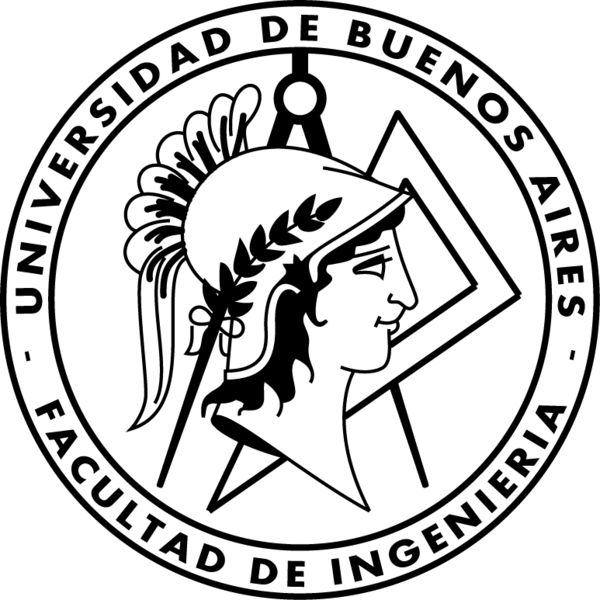
\includegraphics[scale=1]{res/fiuba_logo.png} 
\end{figure}
\begin{center}\normalsize{Facultad de Ingeniería, Universidad de Buenos Aires}\end{center}
\newpage

\tableofcontents
\newpage

% *** RESOLUCION ***
% Some settings for coding style
\lstset{
    basicstyle=\linespread{0.9}\ttfamily\footnotesize,
    frame=single,
    frameround=tttt,
    numbers=left,
    numberstyle=\tiny,
    linewidth=14cm,
    literate=
      {á}{{\'a}}1 {é}{{\'e}}1 {í}{{\'i}}1 {ó}{{\'o}}1 {ú}{{\'u}}1
      {Á}{{\'A}}1 {É}{{\'E}}1 {Í}{{\'I}}1 {Ó}{{\'O}}1 {Ú}{{\'U}}1
      {à}{{\`a}}1 {è}{{\`e}}1 {ì}{{\`i}}1 {ò}{{\`o}}1 {ù}{{\`u}}1
      {À}{{\`A}}1 {È}{{\'E}}1 {Ì}{{\`I}}1 {Ò}{{\`O}}1 {Ù}{{\`U}}1
      {ä}{{\"a}}1 {ë}{{\"e}}1 {ï}{{\"i}}1 {ö}{{\"o}}1 {ü}{{\"u}}1
      {Ä}{{\"A}}1 {Ë}{{\"E}}1 {Ï}{{\"I}}1 {Ö}{{\"O}}1 {Ü}{{\"U}}1
      {â}{{\^a}}1 {ê}{{\^e}}1 {î}{{\^i}}1 {ô}{{\^o}}1 {û}{{\^u}}1
      {Â}{{\^A}}1 {Ê}{{\^E}}1 {Î}{{\^I}}1 {Ô}{{\^O}}1 {Û}{{\^U}}1
      {œ}{{\oe}}1 {Œ}{{\OE}}1 {æ}{{\ae}}1 {Æ}{{\AE}}1 {ß}{{\ss}}1
      {ű}{{\H{u}}}1 {Ű}{{\H{U}}}1 {ő}{{\H{o}}}1 {Ő}{{\H{O}}}1
      {ç}{{\c c}}1 {Ç}{{\c C}}1 {ø}{{\o}}1 {å}{{\r a}}1 {Å}{{\r A}}1
      {€}{{\euro}}1 {£}{{\pounds}}1 {«}{{\guillemotleft}}1
      {»}{{\guillemotright}}1 {ñ}{{\~n}}1 {Ñ}{{\~N}}1 {¿}{{?`}}1
}
\part{Resolución}
\section{Parte 1: Un juego de batalla naval}


\newpage
\section{Parte 2: Sabotaje!}

\subsection{Análisis preliminar y consideraciones previas}
El problema planteado implica un conocimiento de redes de flujo. Una definición con la que trabajaremos es la siguiente: se entiende como red de flujo a un grafo dirigido con aristas pesadas. Llamamos al peso de cada arista la capacidad entre los dos vértices que conecta. Las redes de flujo cumplen las condiciones:
\begin{itemize}
    \item Existe un único vértice con únicamente aristas salientes a él, sin aristas entrantes, llamado fuente.
    \item Existe un único vértice con únicamente aristas entrantes a él, sin aristas salientes, llamado sumidero.
    \item Todos los demás vértices cumplen la condición de que la capcidad entrante, es decir, la sumatoria de todas sus aristas que terminan en este vértice, es igual a la capcidad saliente, la sumatoria de todas las aristas con fuente en este vértice.
\end{itemize}

La última condición implica una conservación de la capacidad: en la red, todos los nodos intermedios entre la fuente y el sumidero tienen una capacidad neta nula, solo transportan capacidad entre las puntas, sin crear o destruir capacidad adicional.

Las redes de flujo modelan problemas en donde, valga la redundancia, fluye una cantidad apreciable de un bien sobre ciertas vías (los ejes o aristas), en donde cada vértice marca una intersección donde se puede redirigir la dirección del flujo. Las aplicaciones más comunes es en líquidos en cañerías en un problema de hidráulica, corriente eléctrica en un circuito, o el tránsito en un sistema de autovías, entre otros.
 
Definimos flujo de un eje como la cantidad de ese valor modelado (corriente, líquido, tránsito), que está circulando actualmente entre los nodos determinados. Este valor, por supuesto, debe ser menor a la capacidad total de ese eje, y también debe cumplir la condición de conservación: el flujo entrante a un nodo es igual al saliente.

El cuello de botella, \textit{bottleneck}, de un camino entre fuente y sumidero es la capacidad mínima de todos los ejes del camino. Este valor es el flujo máximo que puede llegar a circular por ese camino, debido a la condición anterior de que el flujo no puede ser mayor a las capacidades de los ejes por el que pasa.

\begin{figure}
    \centering
    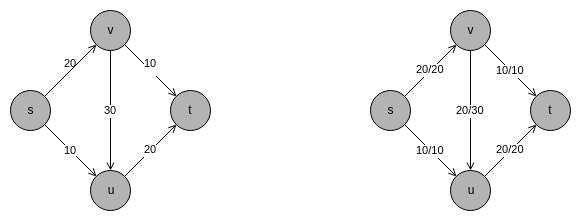
\includegraphics[scale=0.5]{res/flow_network.png}
    \caption{Red de flujo con capacidades totales y con flujo/capacidad total}
\end{figure}

Leyendo el enunciado se toman varias suposiciones. La más importante es que la red que tenemos que proteger es una red de flujo de manera tal que cumpla con la definición dada anteriormente. Lo segundo es la interpretación de "los saboteadores quieren hacer el máximo daño posible" del enunciado. Se entiende que los saboteadores actúan de manera completamente óptima: Primero sabotearán el eje más importante de la red (a definir más adelante), y luego, el segundo más importante, que será el eje más importante de la red de flujo resultante al tener inoperante el primer eje. Dicho de otra manera, los saboteadores atacan como segundo eje al que sería más importante en una red de flujo que no contenga al primer eje saboteado.

No está de más aclarar también que la solución implementada es óptima y termina con el orden determinado únicamente cuando las capacidades de los ejes son números enteros. 

\subsection{Algoritmo propuesto}

El problema se resume en determinar las dos aristas más importantes de la red. Es sencillo de ver que si encontramos el flujo máximo que puede pasar por nuestra red, las aristas más importantes serán las que mayor flujo pasen por ellas. El algoritmo a proponer se resume a este concepto, hallamos el flujo máximo de la red, y luego iteramos sobre todas las aristas de la red y detectamos las de mayor flujo. El flujo máximo se calcula por el algoritmo de Ford Fulkerson, con la búsqueda de caminos fuente-sumidero usando DFS. 

El algoritmo implementado es óptimo gracias a la garantía de que el flujo máximo encontrado es óptimo, Ford Fulkerson determina la mayor cantidad de flujo pasable por la red. Sabiendo que los flujos son óptimos, el resultado de iterar sobre ellos devolverá las aristas más importantes también será óptimo.

\begin{algorithm}
    \KwData{$G$: red de flujo a determinar vulnerabilidades, $n$: cantidad de ejes a proteger}
    \KwResult{$vul$: lista de ejes a proteger}
    \BlankLine

    $R$ $\leftarrow$ FordFulkerson(G); // Grafo residual
    
    vul $\leftarrow$ [];

    \While{$vul.length < n$}{
        \ForEach{$e \in E(R)$}{
            \If{$vul.length < n$}{
                vul.append(e);
            } \ElseIf{$e.flow > min(vul)$}{
                vul.remove(min(vul));

                vul.append(e);
            }
        }
    }
    return $vul$;

    \caption{Pseudocódigo del algoritmo propuesto}
\end{algorithm}

La complejidad del algoritmo está acotada por Ford Fulkerson, de orden $O(mC)$, siendo $m$ la cantidad de vértices de la red, y $C$ la capacidad saliente de la fuente. El hallado de los ejes más importantes de la red es una búsqueda lineal sobre las mismas, $O(n) = O(2m) = O(m)$. Se podría ver como una reducción sobre Ford Fulkerson: se está usando el algoritmo de flujo máximo como una caja negra, y simplemente iterando sobre sus resultados (transformación de valores de salida) para determinar la solución a nuestro problema.

La complejidad es calculada de esta manera gracias a la suposición de que las capacidades son valores enteros. El algoritmo de Ford Fulkerson utiliza esta suposición para dar su propia cota de complejidad. De ser las capacidades un valor fraccionario, ni siquiera se podría garantizar la terminación del algoritmo, debido a que en el peor caso Ford Fulkerson podría llegar a aumentar su flujo de a cantidades arbitrariamente pequeñas hasta llegar al máximo.

Analizando los flujos máximos antes y después del sabotaje podemos apreciar que el flujo no necesariamente difiere en la cantidad exacta de los flujos de las aristas saboteadas. Si borramos esas aristas, el flujo puede ser redirigido y tomar una dirección con capacidad disponible que antes no hacía porque simplemente no era conveniente.

\subsection{Implementación}

Se implementó el algoritmo propuesto (junto con Ford Fulkerson) en Nodejs. Para correr el código, asegurarse de contar con una versión de Node $>=$ 8.0, correr \textit{npm i}, y luego \textit{npm start}.


\end{document}
